\chapter{平等の要求}








\section{オランプ・ドゥ・グージュ『女性および女性市民の権利宣言』(1791)}

オランプ・ドゥ・グージュ (Olympe de Gouges, 1748--1793)。


出典:オリヴィエ・ブラン『女の人権宣言:フランス革命とオランプ・ドゥ・グージュの生涯』、辻村みよ子訳、岩波書店、1995。

\subsection*{序文}

母親、娘、姉妹たち、国民の女性代表者たちは、国民議会の構成員となることを要求する。そして、女性の諸権利に対する無知、忘却または軽視が、公の不幸と政府の腐敗の唯一の原因であることを考慮して、女性の譲り渡すことのできない神聖な自然的権利を、厳粛な宣言において提示することを決意した。この宣言が、社会のすべての構成員に絶えず示され、かれらの権利と義務を不断に想起させるように。女性の権力と男性の権力の行為が、すべての政治制度の目的とつねに比較されうることで一層尊重されるように。女性市民の要求が、以後、簡潔で争いのない原理に基づくことによって、つねに憲法と良俗の維持と万人の幸福に向かうように。

こうして、母性の苦痛のなかにある、美しさと勇気とに優れた女性が、最高存在の前に、かつ、その庇護のもとに、以下のような女性および女性市民の権利を承認し、宣言する。

\begin{description}

 \item[第一条] 女性は、自由なものとして生まれ、かつ権利において男性と平等なものとして生存する。社会的差別は、共同の利益に基づくのでなければ、設けることができない。

 \item[第二条] あらゆる政治的結合の目的は、女性および男性の、時効によって消滅することのない自然的な諸権利の保全にある。これらの諸権利とは、自由、所有、安全、そしてとりわけ圧政への抵抗である。

 \item[第三条] あらゆる主権の淵源は、本質的に国民にあり、国民とは、女性と男性との結合にほかならない。いかなる団体も、いかなる個人も、国民から明示的に発しない権威を行使することはできない。
……

 \end{description}



 \begin{figure}[htbp]
   \centering
     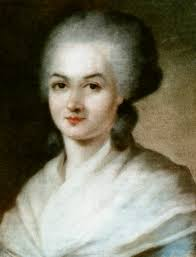
\includegraphics[width=50mm]{images/gouges.jpg}
   \caption{オランプ・ドゥ・グージュ}
 \end{figure}








\section{ウルストンクラーフト『女性の権利の擁護』 (1792)}


メアリ・ウルストンクラフト。(Mary Wollstonecraft, 1759--97)。

典拠:メアリ・ウルストンクラーフト、白井堯子訳(1980)『女性の権利の擁護』、未来社



\subsection{}

  ルソーは次のように言明する。女性は、瞬時といえども、自分は独立していると感じてはならないと。そして、女性は、\kenten{生まれつき}持っているずるさを発揮するためには恐怖によって支配されるべきであり、自分を欲望の一層魅惑的な対象にするために、すなわち、男性がくつろぎたいと思う時にはいつでも彼の\kenten{もっとも優しい}お相手になれるように、コケティッシュな奴隷にならねばならないと。彼は更に議論を進め{\——}自然の命ずるところに従ったふりをして{\——}次のことをほのめかす。誠実と不屈の精神は、すべての人間的美徳の基礎であるが、女性の性格については、服従を厳しく叩きこむことが大事な教育なのだから、誠実や不屈の精神はほどほどに教えるべきだと。

  何と馬鹿げたこと! 男性の高慢と好色のために、この問題の上には、こんなにもひどく煙が立ち込めてしまった。これを吹き払うに足りる程の知力を持った偉大な男性が、いつの日にか出現するであろうか! たとえ、女性には生まれつき男性には及ばない点があるとしても、彼女たちの美徳は、程度においてはともあれ、質においては男性と同じでなければならないのだ。さもなければ、美徳は相対的な概念となってしまう。それ故に、女性の行為は、男性と同じ原理の上に築かれ、同じ目的を持たなければならない。(pp. 55-56)


\subsection{}

  恋愛に重きを置かずに論を進めるのは、情操や繊細な感情に対して大逆罪を犯すものであることは承知している。だが私は、真理の持っている単純な言葉を語りたいし、心よりもむしろ、理性に話しかけたい。この世から恋愛をなくそうと説得に務めることは、セルヴァンテスのドン・キホーテを追い出すことであり、ドン・キホーテと同じように常識に背くことを行うことになろう。しかし乱れ騒ぐ\ruby{情欲}{パッション}を抑えようとする努力は、そしてまた、次元の高い能力を下位に置いてはならぬことを証明しようとする努力は、あるいは、知性が常に冷静に保持すべき大権を奪い取ることは許されないことを証明しようとする努力は、それ程暴論とは思えない。

  青春は、男性にとっても女性にとっても、恋愛の季節である。けれども、思慮に欠けるこうした享楽の時代においても、人生のもっと重要な時代{\——}その時には、熟慮が興奮に代って登場する{\——}のために、準備がなされなければならないのだ。それなのに、ルソーや彼を見習った大抵の男性著述家たちは、女子教育の趣旨はひたすら一つの点{\——}男性を喜ばせる女になること{\——}に向けられるべきである、と熱心に説いてきた。

  このような意見の支持者で、人間性について何らかの知識を持っているような人と議論しよう。彼らは、結婚は生活習慣を根こそぎ変えうるものである、と想像するのであろうか?ただ男性を喜ばせることだけを教えられてきた女性は、彼女の魅力が落日の夕日の如く沈むことを、いずれ知るであろう。夫と毎日鼻を突き合わせてばかりいる時には、また女盛りが過ぎ去った時には、自分の魅力が夫の心をあまりつかむことができなくなるということを、やがて知るだろう。その時になって女性は、他人に頼らず自分で楽しみを見出していくために十分な、また自分の潜在能力を磨くためにも十分な、本来のエネルギーを持てるであろうか?持てないとなると、別の男性を喜ばせようと試みると考える方が、もっと合理的ではないであろうか?そして新しい愛を獲得する期待から生まれた感情の中で、彼女の愛や自尊心が受けた屈辱を忘れようと考える方が、もっと合理的ではないであろうか? 夫が自分を愛してくれる人ではなくなった時{\——}その時は必ずや来るであろう{\——}には、彼を喜ばせたいという彼女の願いは暗礁に乗り上げるか、あるいは、悲嘆の源となるであろう。そして恋愛、恐らく、あらゆる\ruby{情熱}{パッション}のうちで最も移ろいやすい愛は、嫉妬や空しさに席を譲るのである。

  私は今、何かの信念、もしくは偏見によって抑制された女性について語る。このような女性は不義密通というようなことは大嫌いであろうが、それにもかかわらず、彼女たちだって夫からひどく冷淡にあしらわれているのがはっきりした時には、他の男性からちやほやされることを望むのだ。そうでなければ、夫と意気投合した魂が享受した過ぎし日の幸福を夢見ながら、毎日、毎週を過ごし、ついには、彼女たちの健康は蝕まれ、精神は不満のために傷つくのだ。そうだとすると、男性を喜ばせるという大変な技術を学ぶことは、そんなに必要な学習でありえようか?それは、ただ情婦にとって役に立つだけである。清純な妻や、真面目な母は、人を喜ばせる能力は彼女の美徳を磨くことによってのみ生まれる、と考えるべきであり、夫の愛情を、彼女の仕事を容易にし彼女の人生をより幸福なものにするための励ましの一つとしてだけ考えるべきである。{\——}しかも、愛されていようが無視されていようが、彼女の第一の望みは、自分自身を尊敬に値するものに成長させることであって、幸福のすべてを、彼女と同じように弱さを持っている人に賭けてはならない。(pp.58-60)



\subsection{}



階級というとんでもない区別は、この世の人間を、好色な専制支配者とずるくて猜疑心の強い被支配者に分割することによって分明を一つの呪いにしている。またこの区別は、あらゆる階級の人びとを、殆ど同じように堕落させてもいるのだ。というのは、人間は、相手の生活上の義務の履行に対して尊敬を払うのではなく、相手の地位に対して尊敬を払うからである。愛情は美徳に対する自然の報酬なのだが、義務が果されていない時には、愛情は美徳を強めるだけの十分な力を得ることはできない。しかし、それでも男性には、そこからはい出して一人で思い切って考え、行動することのできる抜穴がある。だが、女性が、そこからはい出すのは至難の業だ。というのは、女性にだけ伴うあの困難を克服せねばならないし、それには超人的な力を必要とするのだから。

真に社会全体の利益を考える立法者は、美徳を持つということがあらゆる人間の関心の的となるように、常に努力する。そうすれば、個人の美徳が、すなわち公共の幸福を築くようになるのだから、自然の秩序に基づく全体は、皆が同じ目標に向うという傾向を持つことによって、強固なものとなる。しかし、女性が個人としての美徳、あるいは公的な美徳を持つことができるかどうかは、甚だ怪しい。というのは、ルソーや、おびただしい男性の著述家たちは、女性は一生の間、厳しい束縛、正義作法という束縛に従うべきだ、と主張しているからである。何故女性を、礼儀作法に従わせるのか?{\——}もし女性がもっと高貴な動機によって行動しうるとするならば、またもし女性が不滅の魂を保持するとするならば、何故無意味な礼儀作法に従わせるのか?

砂糖は、生きた人間の血からいつも作られるべきなのか?

男性の盃を甘くするだけのために、人類の半分である女性は、哀れなアフリカの奴隷と同じように偏見に従うべきなのか?

原理は彼女たちを確実に守るであろうが、偏見は彼女たちを野獣のような惨めな状態にしてしまうのだ。偏見に従わせることは、間接的に女性の理性を否定することではないか?
何故ならば、理性を与えられていても、それを使用しない方がよいといわれる時には、そのような理性はおもちゃ同然だからである。(273-274)


\subsection{}

  閉鎖的な教育によってしばしば形成されるあの女性の愚かな性格のもう一つの例は、いみじくも\kenten{センチメンタル}と呼ばれてきた、ロマンティックにものを考える傾向である。

女性は無知故に自分の気分に支配されやすいし、恋愛における幸福を求めることだけを教えられているので、官能的な感情に磨きをかけたり、恥ずかしげもなく人生の義務を忘れさせるあの\ruby{情熱}{パッション}について夢のような考えを抱く。そして、彼女たちは、このようなことに得々となって磨きをかけている最中に、転落の路を辿り、現実に悪徳を行うようになるのだ。

こういう女性は、愚劣な小説家が描いた空想を喜ぶような人たちだ。愚劣な小説家というものは、人間性についてほとんど何も知らないくせに、陳腐な物語を作り上げ、淫らな場面を描きだす。それらは、すべてセンチメンタルな戯言で詳述されており、いずれも趣味を俗悪化させたり、日常の義務から心をそらせるのに役立つ。……

女性はすべての政治的な特権を否定され、また既婚女性の場合には、刑事事件の場合を除き市民的な存在とも認められていないので、当然、彼女たちは社会全体の利益などはそっちのけにしてごく小さな一部の利益に注意を払う。……女性の生活における大きな仕事は、人を喜ばせることになっている。そして彼女たちは政治的にもまた市民としても抑圧されて大事な事柄にかかわれないようにされているので、感傷こそが大事件になり、もっと広い範囲に知性を働かすことが許されているならば問題にもしないようなことに、あれこれと頭を使う。

……偉大なものを把握する能力を備えていない彼女たちが、歴史書を紐解くなんていうことはまったく無意味な仕事だと考えたり、知性に訴えるような論文は死ぬ程退屈で、およそちんぷんかんぷんだと思うのは、驚くべきことだろうか? だから、彼女たちの楽しみといえば、必然的に小説になってしまうのだ。しかし私が小説を声高く非難するのは、知性を働かせ想像力を抑えるような著作と比較した場合である。{\——}というのは精神は、その思考力をわずかでも働かせれば、ある程度広やかになり、少しは強くもなるに違いないから、私は、どんな本であろうと読書をすることは、空っぽな頭をそのままにしておくよりはましだと思っているのだ。さらに述べれば、想像力におもねるに過ぎない作品であっても、それを読むことは、デリカシーとは似ても似つかぬあの淫らな欲望を満足させるよりは、少しは読者を高めるであろうから。(pp. 342-343)



 \begin{figure}[htbp]
   \centering
     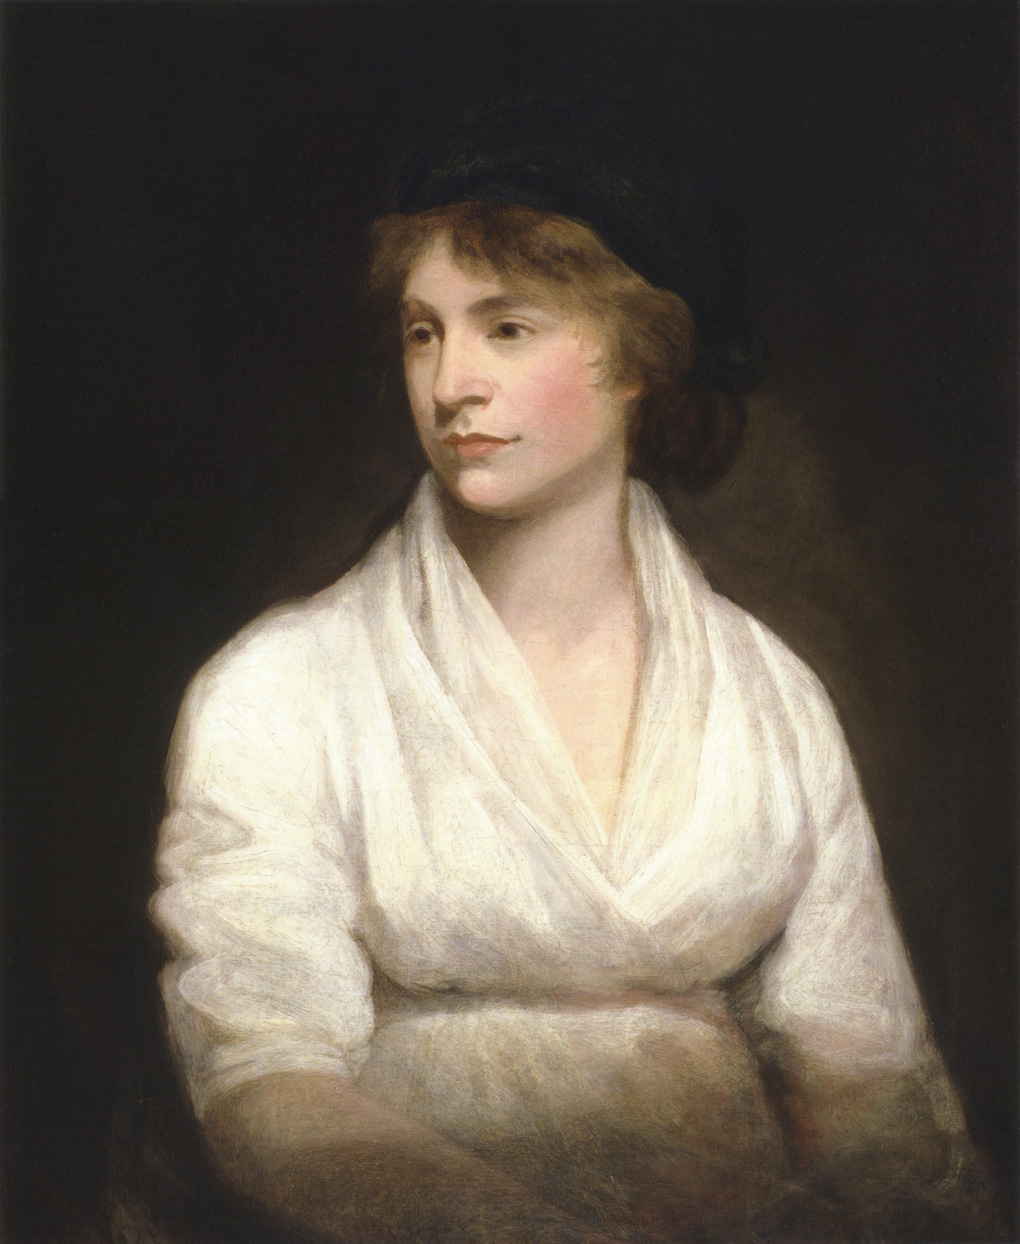
\includegraphics[width=50mm]{images/Marywollstonecraft.jpg}
   \caption{ウルストンクラフト}
 \end{figure}



\section{ゴドウィン『政治的正義』 (1793)}

ウィリアム・ゴドウィン (Wiliam Godwin, 1756--1836)。

出典:ウィリアム・ゴドウィン『政治的正義』、加藤一夫訳、春秋社、1930。


\subsection{}



人類の利益に後見することのできるあれやこれやの物資を諸君の財産または私の財産と考えてよいか悪いかを決定する必然の標準はなんであるか? この疑問に対しては、ただ一つの答があるだけである{\——}それは正義である。そこで我々はふたたび正義の原理に立ち戻って論じよう。


財産のある品目、仮に一塊のパンは、正当に誰のものであるか? それを最も多く要する者に属するか、もしくはそれを所有することによって最も多くの利益を与えられる者に属するかである。ここに飢餓に迫られている6人の人がいるとする。そして一塊のパンは、それだけを考察すれば、彼等のすべての渇望を満足させることができる。この一塊のパンが持っているかかる性質を利用しようと要求しても差し支えない人はいったい誰であるか? それは恐らく鏡台すべてである。しかも長子相続の法律はそれを長子だけに与える。しかし正義はこの判定を明証するか? 相異なった国々の法律は、財産を無数の相異なった方法で処理する。しかし理性に最も一致する方法は一つしかありえないのである。

今述べたような場合よりも更に有力な場合をいくらでも持ち出すことができる。私は100個のパン塊を持っている。そして隣の街には、餓死に瀕していて、これらのパン塊が一つあればその生命をとりとめることができるというような貧しい人がいる。もし私がこの一塊のパンを彼に与えないなら、私は不正ではないか? もし私がそれを分け与えるなら、私は正義の要求に応じているのではないか? その一塊のパンは正当に誰に属しているのか?(432-433)



\subsection{}

犯罪の多産的な根源は、一人の人間が他の人間の欠いているとろのものを豊に所有しているというこの一つの事情に損するのである。我々、我々の心の性質を変革するのでなければ、この一つの事情が、心の境遇の性質上、知覚に強くもたらされた場合に、それによって我々の心が力強く影響されないよう防ぐことはできないのである。……


暴力は独占から生じた。それは野蛮人の間にあっては、貪慾が供給を凌いだ場合や、もしくは情欲が欲望の対象の現出によって燃やされた場合に、偶然に持ち上がったものであろう。しかしそれは、理性および文明が進歩するに従って、段々と消滅して行ったであろう、蓄積された財産がそれ自体の支配権を据えて依頼、すべては一党の力と狡猾とに対する他党の力と狡猾との公然とした争いである。この場合、困窮した者等の乱暴な早まった闘争は、疑いもなく悪である。彼らは、朋党の成功を専念しながら、かえってその朋党の失敗を招くようなことになるのである。彼等は心理の勝利を長引かすようになる。しかし真の犯罪は、自分のことだけ考えて、他人の利益を軽蔑している人々の、悪意あるかつ偏頗な性質にあるのである。そして富者は御多分に漏れてはいない。(445)


\subsection{}



この同棲の問題は、結婚の問題を含んでいるから特に興味がある。……同棲は心の独立した進歩を阻止するから悪であるだけではない。それは人間の不完全および嗜好と矛盾している。二人の人間の嗜好および欲求がいかなる長い期間にわたっても一致するように期待することは馬鹿げている。彼等を一緒に行動したり生活したりするように強いることは、口論や邪魔や不幸の幾分かの不可避な部分に彼等を服従さすことである。人間が絶対的完全の標準に達することを誤った限り、これはそうならざるをえないのである。私は一生涯の間伴侶を持たなければならないという仮定は、不徳の錯綜の結果である。それは臆病さの指図であって、剛毅の指図ではない。それは、功績に相当しない何物かのために愛されかつ尊敬されたいという欲望から流れ出るのである。

しかしヨーロッパ諸国で実行されているような結婚の悪は、これよりも一層深い所に存在している。この習慣は、無思慮なロマンチックな男女の青年が一緒になるために、しばらくの間、幻想に満ちた事情の下において、互いに会うこと、それから互いに永遠の愛着を誓いあうことにある。これの結果はどうなるか? ほとんどあらゆる実例において、彼等は自分が欺かれていることを知る。彼等は取り返しのつかない錯誤をもっともよく利用することに従う。彼等は、虚偽の阿呆になるための、想像しえる最も強い誘惑を与えられる。彼等は現実に対して眼を閉じることをもっとも賢い製作だと考えるようになる。もしいかなる理知の壊敗によってでも、彼等が自らを説服して、自分等の最初の不熟な意見では自分等の交りは正しかったのだと信ずることができるなら幸福だ。結婚の制度は詭計の制度である。そして自分の生活の日々の事件において自分の判断を慎重に誤りに導く人々は、いつも他のあらゆる事件において不具な判断をしなければならないのである。我々は、自分の錯覚が発見されるや否や、それを減少させるべきである。しかし我々は、自分の研究を阻止して、最も魅力ある賞讃すべき対象に対して自分の眼を閉じるように教えられるのである。結婚は法律であり、すべての法律の中の最も悪いものである。一緒になれば我々に最大の改善を与えるべき人間について一人の女の価値と他の女の欠点について、我々の理解がどういう事を告げようとも、我々は何が法律であるこかを考察するように強いられて、何が正義であるかを考察するようには強いられないのである。

これに付け加えよ。結婚は財産上の事件であって、すべての財産の中の最も悪いものであるということを。二人の人間が人定制度によって我々自身の心の指図に従うことを禁じられる限り、偏見は活きて溌剌としている。私が一人の女を自分自身に独占しようと努めたり、私の隣人に、自らのすぐれた功績を証明しかつそれの結実を刈り集めることを禁じようと努めたりする限り、私はすべての独占の中の最も忌しいものについて罪があるのである。この想像的褒賞を、人々は不断の嫉妬をもって注意する。そして一人の人間は出し抜きを行う自分の欲望や能力が振り起されるのを知るだろう、他の人間が彼の希望を空しくしたりするために振り起されるのと同じほどに。この社会状態が継続する限り、博愛は無数の方法で妨げられたり阻止されたりするであろう。そして依然として増大する弊害の流れは流れ続けるであろう。

結婚の廃止には悪は伴わないだろう。我々はそれを獣的な欲望や堕落として心に抱きがちである。しかし実際にこの場合には他の場合においてのように、我々の不徳を抑止するために作られた成文法律は、その不徳を刺激したり増やしたりする。言うまでもなく、平等な財産状態においては奢侈に対する趣味を破壊する正義および幸福の感情は、同じように我々のあらゆる種類の過度の欲望を減少さすだろう。そして我々を導いて普遍的に官能の快楽よりも理智の快楽を選ばせるであろう。……(469-471)



 \begin{figure}[htbp]
   \centering
     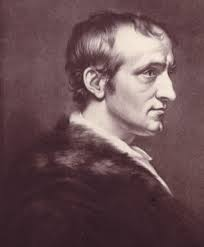
\includegraphics[width=50mm]{images/godwin.jpg}
   \caption{ゴドウィン}
 \end{figure}



\section{マルサス『人口論』(1798)}



典拠:マルサス『人口論』、永井義雄訳、中公文庫、1973



\subsection{}




現在、つぎのようなおおきな問題が論争中である、といわれてきている。人間はこれから加速度的に、無限の、これまで考えられたことにないほどの改善に向かって、前進を開始するであろうか、あるいは、幸福と不幸とのあいだの永遠の往復反復運動を運命づけられており、あらゆる努力にもかかわらず、念願する目標からなおはかりしれないほどの距離にとどまっているであろうか、という問題である。(17)



わたくしは、二つの公準をおいてもさしつかないであろうと考える。

第一、食糧は人間の生存に必要であること。

第二、両性間の情念は必然であり、ほぼ現在の状態のままでありつづけるとおもわれること。


……そこで、わたくしの公準が承認されたものと考えて、わたくしは次のように述べる。人口の方は、人間のための生活資料を生産する地球の力よりも、かぎりなくおおきい、と。

人口は、制限されなければ、等比級数的に増大する。生活資料は、等差級数的にしか増大しない。数字をほんのすこしでもしれば、第一の力が、第二の力にくらべて巨大なことが、わかるだろう。

食糧を人間の生命に必要なものとしている、あのわれわれの本性の法則にしたがって、これら二つのひとしくない力の結果が、ひとしいものに維持されなければならない。……


% このことは、生存することの困難さに起因する、人口にたいする強力かつ不断に作用する制限を意味する。この困難さは、どこかあるところにふりかからなければならないし、また必然的に、


動物および植物の王国全体に、自然は、生命の種子をもっと気前のよい、寛大な手でまきちらしてきた。自然は、それらをそだてるのに必要な空間と養分とについては、比較的、物惜しみしてきた。治城のことの地点にふくまれている生命の芽は、豊富な食糧と、ひろまることのできる豊富な余地とがあれば、数千年が経過するうちに、数百万の世界をみたすであろう。必然、すなわちあの厳然とした、すべてを支配する自然の法則は、さだまった限界内にかれらを制限している。植物および動物は、この偉大な制限的法則のもとで、ちいさくなっている。そして人類は、理性のいかなる努力によっても、それらからのがれることができない。植物および動物のあいだにおいては、その結果は、種子の浪費、病気および早死である。人類にといては、不幸と悪徳とである。前者すなわち不幸は、それの絶対に必然的な結果である。悪徳は、きわめておこる確率のたかい結果であって、したがってわれわれは、それがおびただしくひろまっているのを見ている。しかし、おそらく、それは、絶対に必然的な結果とよばれるべきではない。徳性の試練は、悪へのすべての誘惑に抵抗することである。


人口(増加力)と土地の生産(力)との、二つの力のこの自然的不平等、およびそれらの結果をつねにひとしくたもたずにはおかない、われわれの自然のあの偉大な法則は、社会の完成の途上において、わたくしには克服不可能だとおもわれるおおきな困難をなすものである。その他のすべての論点は、これと比較すれば、些細な副次的な問題である。すべての生命あるものを支配しているこの法則のおもみから、人間がのがれることができる道を、わたくしはしらない。どんな幻想的平等も、もっとも徹底したどんな農業上の規制も、一世紀のあいだでさえ、それの圧力を除去することはできないであろう。それだから、この法則は、そのすべての成員が、安楽、幸福および比較的閑暇のうちに生活し、そしてみずからと家族とに生存手段を提供することになんの不安もかじないような社会の存在可能性にたいして、決定的な反証であるようにおもわれる。

したがって、もしそれらの前提がただしければ、論議は、人類の大多数の完成可能性にたいして、反対の結論になる。(23-25)



 \begin{figure}[htbp]
   \centering
     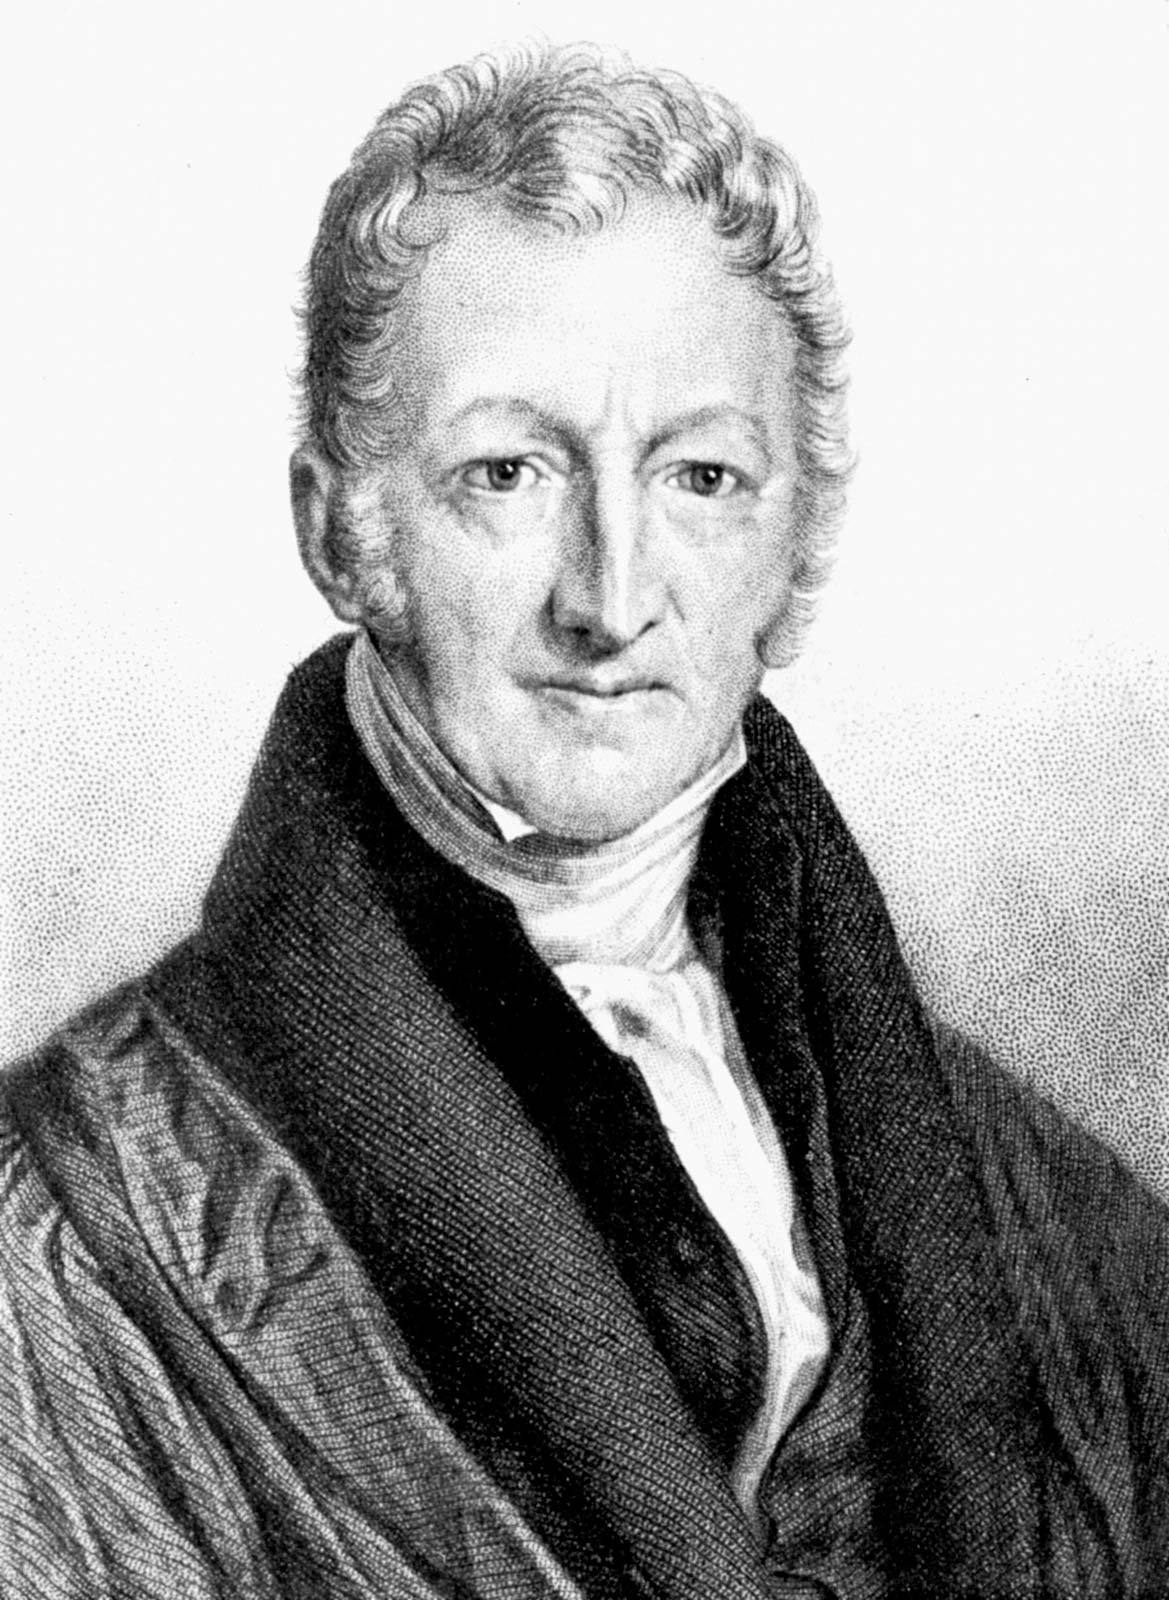
\includegraphics[width=50mm]{images/marthus.jpg}
   \caption{マルサス}
 \end{figure}



\section{推薦図書}





\begin{itemize}
\item 水田珠江(1973)『女性解放思想の歩み』岩波書店〔岩波新書(青版)871〕。古典。(江・渡)
\item 辻村みよ子 (1997) 『女性と人権:歴史と理論から学ぶ』、日本評論社。名著。女性解放運動について1冊読むならとりあえずこれ。(江)
\item 奥田暁子・支倉寿子・秋山洋子 (2003)『図説フェミニズム思想史:明日にむかって学ぶ歴史』、ミネルヴァ書房。(江)
\end{itemize}






%%% Local Variables:
%%% mode: japanese-latex
%%% TeX-master: t
%%% coding: utf-8
%%% End:
